\begin{refsection}


\chapter{Introduction}
The fusion energy has been a goal of active pursuit for nearly seventy years.
The core problem for fusion energy development, as compared to fusion based
weaponry, is the problem of confinement. While the sun had successfully
achieved net positive fusion energy through the successful application
gravitational confinement, that approach is unfortunately not practical for
Earth based application. Instead, a wide variety of alternative confinement
strategies have been attempted, broadly separated into magnetic confinement and
inertial confinement. Where as the inertial confinement focuses on short,
repeated pulses of fusion reaction at very high densities driven by enormous
lasers, magnetic confinement focus on using the magnetic field to restrict the
movement of plasma particles long enough to produce net fusion power. Magnetic
confinement fusion has been favored by the majority of the fusion community, in
part because it does not involve high frequency explosions. magnetic
confinement fusion further divides into a number of 'concepts' based on the
magnetic topology used, with the TOKAMAK taking the lead in achieved plasma
temperature and duration. Everything else is commonly refereed to as
'alternative concepts', and this work deals with one of them: the Reversed
Field Pinch (RFP). In particular, confinement, transport, and heating
characteristics of ions in the RFP.

%=============================================
\section{Fusion power and ion confinement}

\section{Reversed Field Pinch, sawtooth, and tearing mode reduction}

/neoclassica\begin{figure}[!htb]
	\centering
	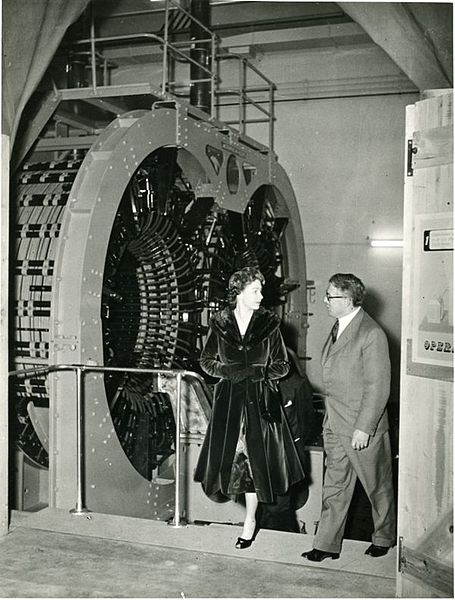
\includegraphics[width = 0.75\linewidth]{./1_Introduction/queen_at_zeta.jpg}
    \label{fig:Queen_at_ZETA}
    \caption[Queen Elizabeth II at the ZETA experiment]{Queen Elizabeth II of Canada and assorted other places, vising ZETA during it's construction in 1957. Photograph by UKAEA}
\end{figure}%

The story of the RFP starts with the Zero Energy Thermonuclear Assembly (ZETA).
Initially built as an extension of the now abandoned toroidal pinch confinement
concept, ZETA was one of the leading fusion experiment of its time, often know
for making and later retracting the first claim of observation of fusion
neutrons, for a time galvanizing world interesting in the imminent arrival of
unlimited energy via fusion. Alas, the claim was made in haste. But persistence
and hard work eventually let scientists at ZETA to discover the spontaneous
reversal of the magnetic field associated with the most stable (quiescent)
period of ZETA's plasmas \cite{Butt_IAEA66,Robinson_IAEA69}. This phenomenon
was explained by J. Taylor in 1974 as a naturally result from the relaxation of
the magnetic topology towards lower energy state \cite{Taylor74}. These were
the foundational documents of the RFP.

\begin{align}\label{eqn:helicity}
	K \equiv \int_{V} \vec{A} \cdot \vec{B} d\tau
\end{align}

Specifically, Taylor posited that in a toroidal plasma of finite resistivity
constrained by a perfectly conducting shell, the magnetic helicity $K$ is
conserved (eqn. \ref{eqn:helicity}). With this constraint, the plasma relaxes
toward a state of minimum magnetic energy characterized by eqn.
\ref{eqn:min_energy_condition}, where $\mu \varpropto K/ \Psi ^2$, is a
constant unrelated to permeability . 

\begin{align}\label{eqn:min_energy_condition}
    \nabla \times \vec{B} = \mu \vec{B}
\end{align}

In cylindrical approximation, the solution to equation
\ref{eqn:min_energy_condition} are Bessel functions (eqn.
\ref{eqn:rfp_solution}) where $B_Z$ reverses in the edge if the plasma current
is high compared to toroidal flux \cite{Taylor74}.

\begin{align}\label{eqn:rfp_solution}
B_z &= B_0J_0(\mu r)\\
B_\theta &= B_0 J_1(\mu r)\\
B_r & = 0
\end{align}

The magnetic topology of atypical RFP is shown in figure
\ref{fig:RFP_geometry}. The relatively low $B_t$ means the RFP have several
advantages over the Tokamak. In the tokamaks, powerful toroidal field coils (TF
coils) are used to generate toroidal flux and keep the safety factor q is kept
above 1 in order to stabilize the plasma. This leads to limits on the toroidal
plasma current depending on the the available coil generated toroidal flux.
This in turns is limited by engineering constrains in terms of magnetic coil
construction. The reversed field pinch avoids these constrains, and
consequently can be constructed with much simpler and cheaper TF coil
arrangements, as well as being more easily reach very high current levels to
take advantage of large Ohmic heating, possibly to ignition levels.

\begin{figure}[!htb]
	\centering
	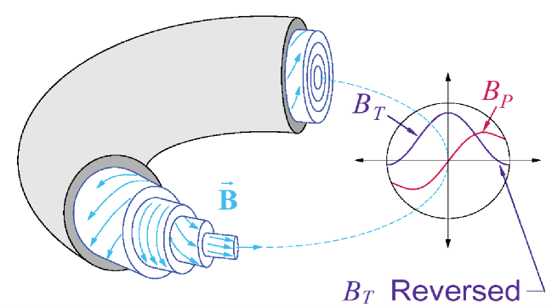
\includegraphics[width = 1.\linewidth]{./1_Introduction/RFP_mag_geometry.png}
	\label{fig:RFP_geometry}
	\caption[RFP magnetic topology]{Illustration of the RFP topology. The most distinct features of the RFP is the similar magnitudes of $B_t$ vs. $B_p$, as well as the fact that $B_p$ reverses direction near the edge.}
\end{figure}%

However, the magnetic topology also poses challenges to the RFP's confinement
characteristics. Taylor noted that the relaxation of the magnetic field is made
possible by the finite resistivity, but did not speculate on the 'method' of
relaxation. Experiments have shown that the relaxation occurs via resistive
tearing mode instabilities which poses a challenge to RFP confinement
characteristics.

\begin{figure}
	\centering
    \label{fig:q_profile}
    
    \caption[Example RPF q profile]{q profile typical of the plasmas studies in this work. Note the closely space resonant surfaces.}

\end{figure}

Research into the RFP configuration led to a series of larger and higher current devices. Currently the leading RFP research devicecs are the Reversed-Field eXperiment\cite{Bartiromo1999RecentExperiment} (RFX) in Padua, Italy, and the Madison Symmetric Torus\cite{Dexter1991} (MST) in Madison, Wisconsin. Comparatively, RFX is capable of driving significantly higher current for a longer duration, where as MST was designed around a close fitting conducting shell to stabilize resistive wall modes. This work is performed on MST, and a more in depth introduction to the device can be found in section \ref{sec:MST}.

%=============================

\begin{figure}[!htb]
	\centering
	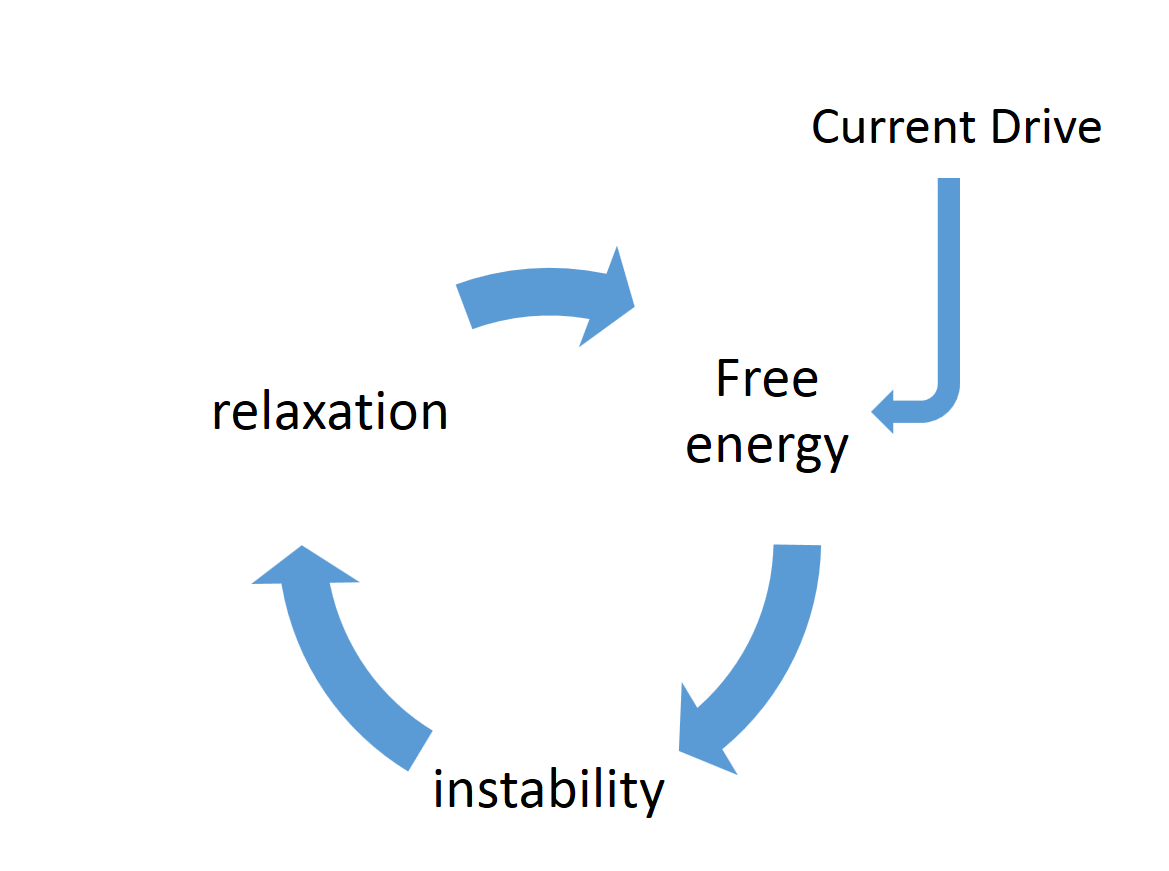
\includegraphics[width = .6\linewidth]{./1_Introduction/the_sawtooth_cycle.PNG}
	\label{fig:sawtooth_cycle}
	\caption[The sawtooth cycle]{The sawtooth cycle that dominates standard RFP plasmas. Improving RFP confinement involves the suppression of this cycle. The PPCD approach involves the suppression of the tearing mode instabilities while inductively driving the plasma current profile relaxation.}
\end{figure}%

The finite resistivity of the plasma allows for the reconnection of the
magnetic field lines and the formation of magnetic islands through tearing mode
instabilities. Tearing modes are unstable at magnetic resonant surfaces where
the safety factor $q \equiv \frac{rB_T}{R_0B_p}$ is a rational number, ie $q =
\frac{m}{n}$ where m and n are integers. The location of these unstable regions
form 'resonant' surfaces that are typically labeled by their m and n numbers.
The RFP have q significantly lower than 1 everywhere, and further decreases
monotonously towards the edge where it will cross 0. An example q profile is
show in figure \ref{fig:q_profile}. This leads to the existence of a large
number of resonant surfaces, especially close to the reversal surface. 

These closely spaced resonant surfaces and the tearing mode instabilities that
they 'host' creates regions of overlapping magnetic islands that turns the
magnetic field stochastic, greatly reducing the confinement characteristics.

The primary drive of the tearing mode instabilities are the current density gradient\cite{Schnack1987Semi-implicitCalculations,Ho1991NonlinearPinches}. Specifically $\nabla\lambda$ where,

\begin{align}
    \lambda &= \frac{J_{\parallel}}{B}\\
    &= \frac{\vec{J}\cdot\vec{B}}{B^2}\nonumber
\end{align}
where $J$ is current, $B$ is magnetic field, and all quantities are flux surface averages. 

In standard RFP operation, the $\lambda$ profile tends to peak in the core of the plasma as the result of current drive, providing free energy to core resonant tearing modes. As the current peaks, the core tearing modes grow and nonlinearly couples to each other, until they are sufficiently large to trigger a violent relaxation event called a sawtooth crash. This redistributes the current profile such that toroidal current in the core decreases while the poloidal current in the edge increases\cite{Terry2004MeasurementTorus}. This effectively flattens the $\lambda$ profile and decreases the drive of the tearing instabilities. But the process repeats as the current profile peaks again in a cycle that is refered to as the sawtooth cycle (fig. \ref{fig:sawtooth_cycle}). Though ion heating is
observed with the sawtooth crashes\cite{Bodin1980Reversed-field-pinchReserarch}, they greatly disrupts
confinement of particles and limit the RFP's viability as a fusion concept.

\begin{figure}[!htb]
	\centering
	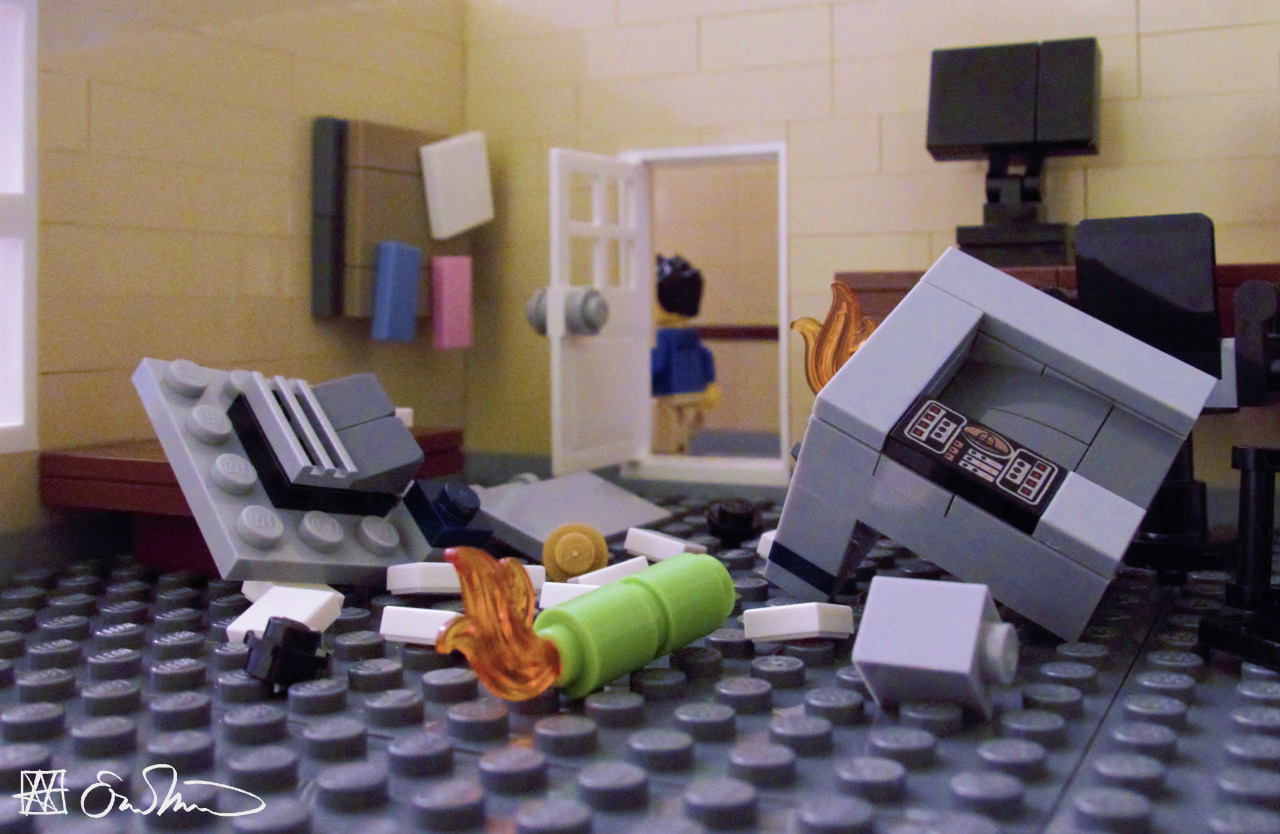
\includegraphics[width = .8\linewidth]{./1_Introduction/violent_relaxation.jpg}
	\label{fig:violet_relaxation}
	\caption[An illustration of violent relaxation]{An artist's impression of a violent relaxation event. By the Lego Grad Student}
\end{figure}%

One successful way of improving confinement on the RFP, therefore, is through the control of $J_{\parallel}$ profile. This is done inductively on MST through a process called Pulsed Parallel Current Drive (PPCD). PPCD can be thought of as 'helping' the plasma to drive parallel current in the edge region, and thereby flattening the $\lambda$ profile\cite{Sarff1995TransportPinch}. In particular, a series of 4 high voltage capacitor banks discharges are used to apply voltage to the toroidal field circuit. This result in a series of 4 poloidal field pulses, which raises $E_{\parallel}$ in the edge. Thus, PPCD is a transient current drive and profiles of the RFP continually evolve during this period. 

With successful applications of PPCD, sawtooth cycles are interrupted which allows a new class of dynamo events called m = 0 bursts to come to the forefront. Details regarding these m=0 bursts is forthcoming in section \ref{sec:m0_intro}. In the meantime it suffice to say that the frequency of these m=0 bursts can be significantly reduced by reversing the applied toroidal electric field in the edge of the plasma\cite{Chapman2001}.

\section{PPCD and it's effect on ion confinement} \label{sec:PPCD_characteristic}

\begin{figure}
    \centering
    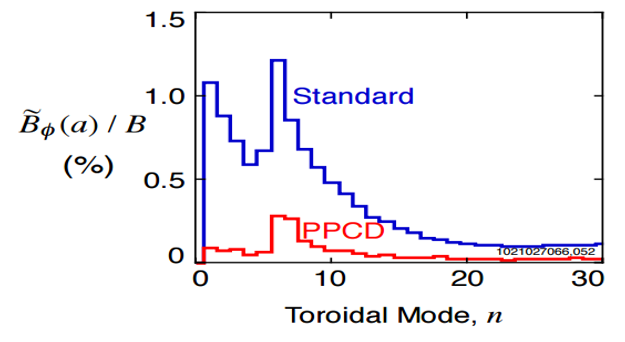
\includegraphics{./1_Introduction/ppcd_fluc.png}
    \caption[Typical tearing mode amplitude in PPCD]{Typical tearing mode amplitude in PPCD [[TODO: remake this plot with matplotlib and my specific data.}
    \label{fig:ppcd_fluc}
\end{figure}

PPCD reduces the tearing mode fluctuation levels significantly as shown in
figure \ref{fig:ppcd_fluc}, and during the period of improved confinement, $T_e$ is known to increase dramatically as compared to standard MST plasma, while $T_i$ is observed to be relatively flat, resulting in temperature differences as high as $T_e \approx 2T_i$ in the core of the plasma. 


At the same time, recent observations shows that drift wave turbulence, likely associated Trapped Electron Mode, continues to be present in PPCD plasma in the edge. 

Though the electron transport properties in PPCD have been studied as part of several thesis previous, the ion transport, particularly the ion thermal transport has not been studied in the same detail. Despite $T_i$ lagging far behind $T_e$, it is thought of as anomalously high in previous estimations. 



%What do I need to get across in this section?
% 0. Reduction in tearing mode fluc levels. 
% 1. Significantly improvement in confinement/reduction in transport terms.
% 2. Separation of ion and electron characteristics.
% 3. Anomalous heating? of the ions?
% 4. Classical impurity particle transport.
% 5. Numerical prediction, especially with regards to the pinch. 
% 6. The persistence of m = 0 bursts. 

 Also Jim Reynolds predicted pinch. Also
significant reduction in fluctuation. Also $T_e$ increase and hot, and have
bursts occasionally, also transport transport transport also stochasticity
decreases, also transient, and some other stuff.


[[Both Santhosh's observation of classical transport but also Reynold's prediction, and Tulio I think.]]


\section{m = 0 bursts in EC and PPCD plasmas}\label{sec:m0_intro}

Bill Young looked at the m = 0 in EC plasmas because he can't look at sawtooth.
Ring like structure, and what not. Also D. Adams made a post for it, measuring
the ring structure, looks good.


[[Bill Young's stuff will be here, as well whatever he cites.]]


\section{Why pursue 1-D classical transport modeling}\label{sec:signpost}
[[Signposting is important]]



Ion transport is important area of research for several reasons in the context
of fusion confinement geometry. The most basic being that it is ion temperature
that is relevant to the rate of fusion reactions. But in particular, there is
long standing disagreement in the field regarding the mechanism behind the well
known anomalous ion heating associated with sawtooth events. At the same time,
there has been confusion about the existence and magnitude of anomalous heating
during periods of improved confinement achieved through parallel current drive.

The RFP geometry suffers from regular global sawtooth events associated with
tearing mode reconnections. While the violent magnetic fluctuations [[Draw
connections with solar and dynamo stuff]]

[Now draw connections with fusion, confinement and whatnot]
\printbibliography%[title={Section bibliography}]

\end{refsection}
